\documentclass[11pt]{article}\usepackage[]{graphicx}\usepackage[]{xcolor}
% maxwidth is the original width if it is less than linewidth
% otherwise use linewidth (to make sure the graphics do not exceed the margin)
\makeatletter
\def\maxwidth{ %
  \ifdim\Gin@nat@width>\linewidth
    \linewidth
  \else
    \Gin@nat@width
  \fi
}
\makeatother

\definecolor{fgcolor}{rgb}{0.345, 0.345, 0.345}
\newcommand{\hlnum}[1]{\textcolor[rgb]{0.686,0.059,0.569}{#1}}%
\newcommand{\hlstr}[1]{\textcolor[rgb]{0.192,0.494,0.8}{#1}}%
\newcommand{\hlcom}[1]{\textcolor[rgb]{0.678,0.584,0.686}{\textit{#1}}}%
\newcommand{\hlopt}[1]{\textcolor[rgb]{0,0,0}{#1}}%
\newcommand{\hlstd}[1]{\textcolor[rgb]{0.345,0.345,0.345}{#1}}%
\newcommand{\hlkwa}[1]{\textcolor[rgb]{0.161,0.373,0.58}{\textbf{#1}}}%
\newcommand{\hlkwb}[1]{\textcolor[rgb]{0.69,0.353,0.396}{#1}}%
\newcommand{\hlkwc}[1]{\textcolor[rgb]{0.333,0.667,0.333}{#1}}%
\newcommand{\hlkwd}[1]{\textcolor[rgb]{0.737,0.353,0.396}{\textbf{#1}}}%
\let\hlipl\hlkwb

\usepackage{framed}
\makeatletter
\newenvironment{kframe}{%
 \def\at@end@of@kframe{}%
 \ifinner\ifhmode%
  \def\at@end@of@kframe{\end{minipage}}%
  \begin{minipage}{\columnwidth}%
 \fi\fi%
 \def\FrameCommand##1{\hskip\@totalleftmargin \hskip-\fboxsep
 \colorbox{shadecolor}{##1}\hskip-\fboxsep
     % There is no \\@totalrightmargin, so:
     \hskip-\linewidth \hskip-\@totalleftmargin \hskip\columnwidth}%
 \MakeFramed {\advance\hsize-\width
   \@totalleftmargin\z@ \linewidth\hsize
   \@setminipage}}%
 {\par\unskip\endMakeFramed%
 \at@end@of@kframe}
\makeatother

\definecolor{shadecolor}{rgb}{.97, .97, .97}
\definecolor{messagecolor}{rgb}{0, 0, 0}
\definecolor{warningcolor}{rgb}{1, 0, 1}
\definecolor{errorcolor}{rgb}{1, 0, 0}
\newenvironment{knitrout}{}{} % an empty environment to be redefined in TeX

\usepackage{alltt}

% Packages for graphics & layout
\usepackage{graphicx}
\usepackage{epstopdf}
\usepackage{subcaption}
\usepackage{booktabs}
\usepackage[a4paper,margin=1in]{geometry}

% Packages for math
\usepackage{amsmath}
\usepackage{amsfonts}
\usepackage{amssymb}

% Package for bibliography
\usepackage{natbib}

\title{Data Analysis Report}
\author{Your Name}
\date{\today}
\IfFileExists{upquote.sty}{\usepackage{upquote}}{}
\begin{document}

\maketitle

\begin{abstract}
This document presents a comprehensive analysis of the data pertaining to...
\end{abstract}

\section{Introduction}
Introduce the context of your data analysis, including the background, objectives, and significance of your study.

\section{Methodology}
Describe the methods used in your analysis. This may include data collection methods, data cleaning and preparation processes, and the statistical or computational techniques applied.

\subsection{Data Collection}
Detail how and where the data was sourced.

\subsection{Data Preparation}
Explain any preprocessing steps like cleaning, normalization, or transformations.

\section{Results}
Present the findings of your analysis. Use tables, graphs, and charts to illustrate your points.
\subsection{Union Density North vs South USA}
\begin{knitrout}
\definecolor{shadecolor}{rgb}{0.969, 0.969, 0.969}\color{fgcolor}
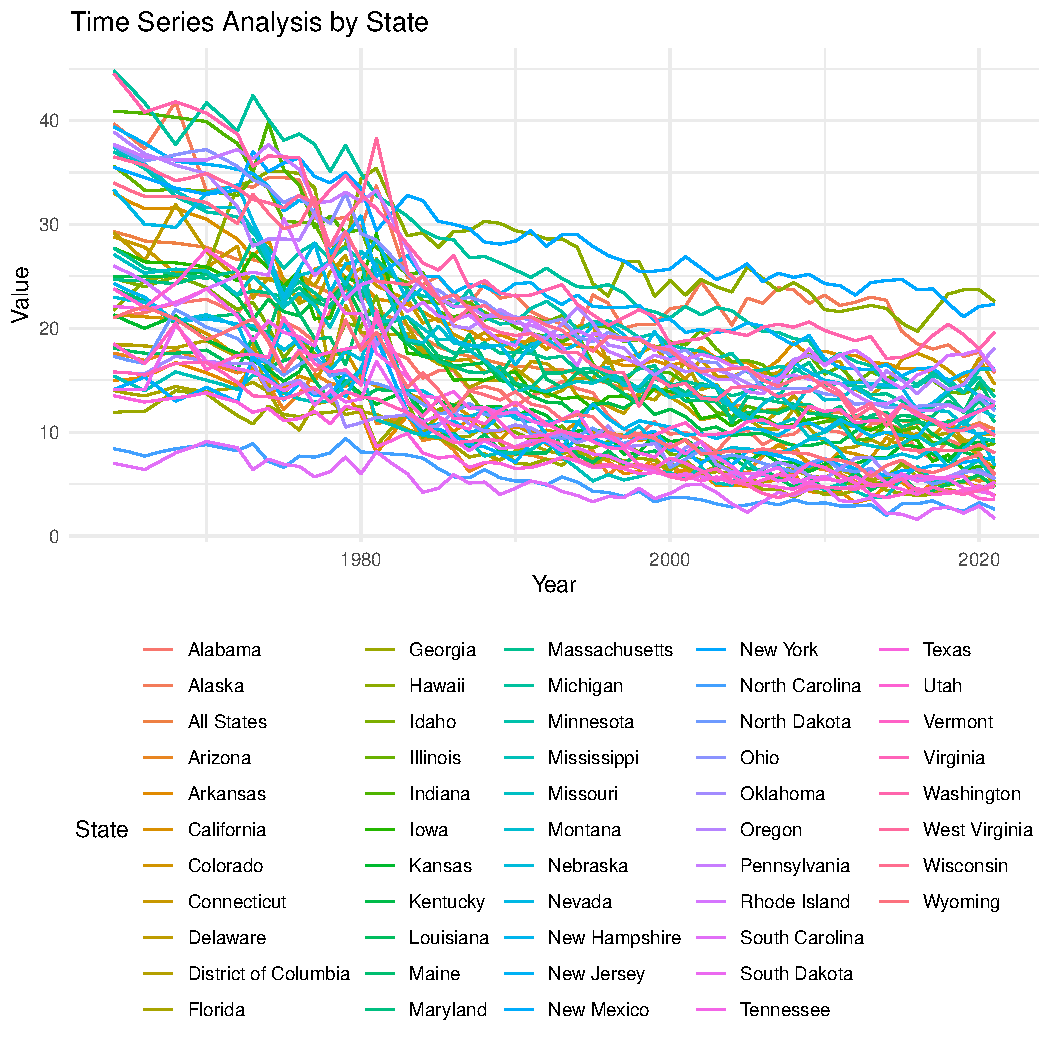
\includegraphics[width=\maxwidth]{figure/unnamed-chunk-1-1} 
\begin{kframe}\begin{verbatim}
##  [1] "Alabama"        "Arkansas"      
##  [3] "Florida"        "Georgia"       
##  [5] "Kentucky"       "Louisiana"     
##  [7] "Mississippi"    "North Carolina"
##  [9] "South Carolina" "Tennessee"     
## [11] "Texas"          "Virginia"      
## [13] "West Virginia"
##  [1] "Connecticut"   "Illinois"     
##  [3] "Indiana"       "Iowa"         
##  [5] "Maine"         "Massachusetts"
##  [7] "Michigan"      "Minnesota"    
##  [9] "New Hampshire" "New Jersey"   
## [11] "New York"      "Ohio"         
## [13] "Pennsylvania"  "Rhode Island" 
## [15] "Vermont"       "Wisconsin"
\end{verbatim}
\end{kframe}
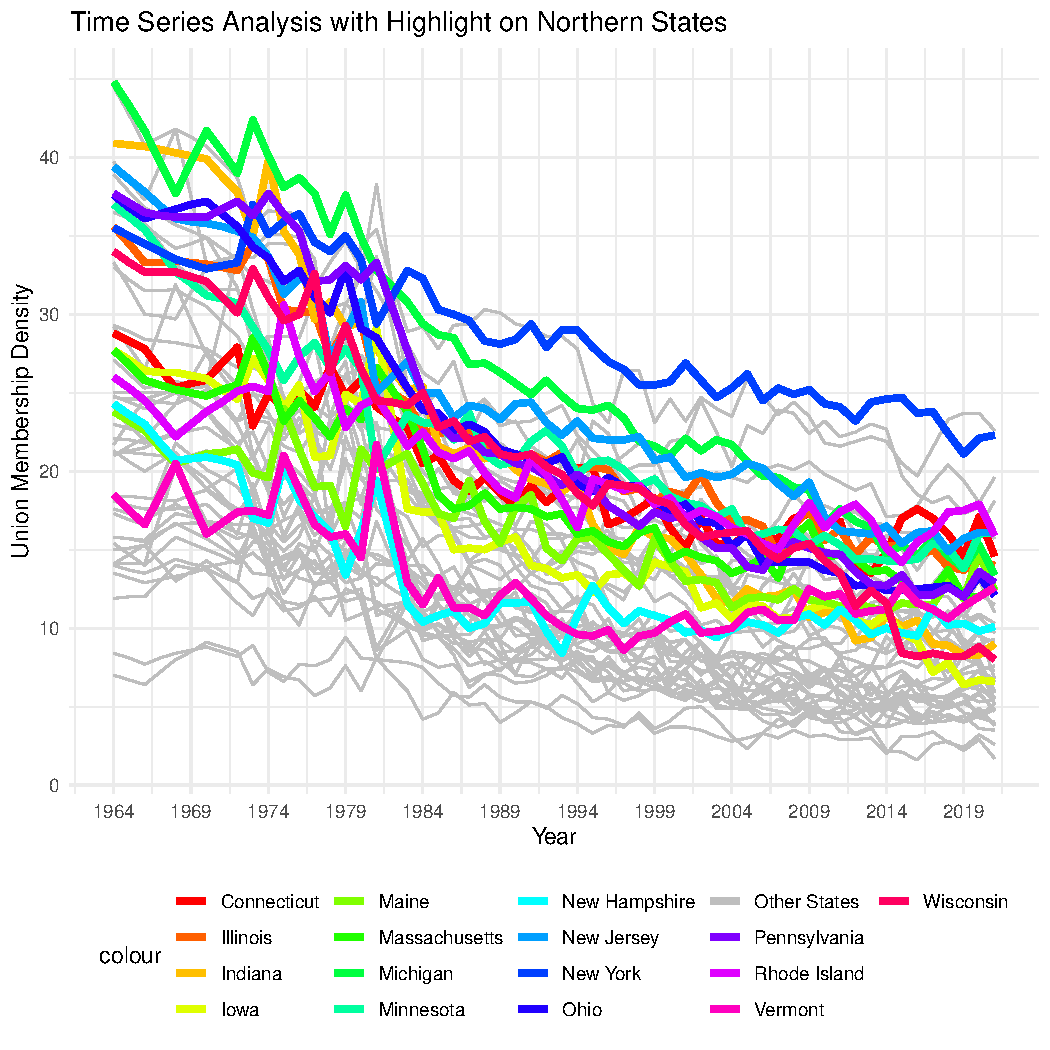
\includegraphics[width=\maxwidth]{figure/unnamed-chunk-1-2} 
\end{knitrout}

\begin{figure}[h!]
\centering
\includegraphics[width=0.5\textwidth]{path/to/your/image/file}
\caption{Caption for your figure.}
\label{fig:yourlabel}
\end{figure}

\begin{table}[h!]
\centering
\begin{tabular}{ccc}
\toprule
Column 1 & Column 2 & Column 3 \\
\midrule
Data 1 & Data 2 & Data 3 \\
Data 4 & Data 5 & Data 6 \\
\bottomrule
\end{tabular}
\caption{Caption for your table.}
\label{tab:yourlabel}
\end{table}

\section{Discussion}
Discuss the implications of your findings, potential limitations of your analysis, and suggestions for future research.

\section{Conclusion}
Summarize the main findings and their relevance to the initial objectives of your study.

\section{References}
\bibliographystyle{plain}
\bibliography{yourbibfile}

\end{document}

